\documentclass[../homework.tex]{subfiles}

\pagestyle{fancy}
\fancyhf{}
\rhead{Hanzhi Zhou}
\lhead{Physics 2415 Homework}
\cfoot{\thepage}

\begin{document}
\subsection{Problem 0.1}
\subsubsection*{a)}
\begin{equation*}
    m = \rho V = \rho \pi R^2 L
\end{equation*}
\subsubsection*{b)}
\begin{equation*}
    \Delta m = \rho \Delta V = \rho \pi R^2 \Delta z
\end{equation*}
\subsubsection*{c)}
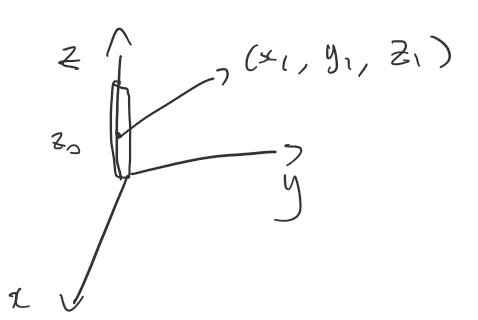
\includegraphics[width=6cm]{sketch.png}
\begin{equation*}
    \vec{r} = x_1\hat{i} + y_1\hat{j} + (z_1 - z_0)\hat{k}
\end{equation*}
\subsubsection*{d)}
\begin{equation*}
    \hat{L} = \sin{\theta}\hat{i} + 0\hat{j} + \cos{\theta}\hat{k}
\end{equation*}
\end{document}